The only traveling "front" wasve $u(x,t) = \Phi(x - ct)$ with $\Phi(-\infty)=1$ and $\Phi(\infty)=0$
is given by:

$$u(x,t) = [1+exp(\frac{x}{\sqrt{6}} - \frac56t)]^{-2}$$

Verify this assertion by deriving the ODE that $\Phi$ has to satisfy and then use a numerical method to
solve it.[Also try analytically!]\\

\begin{solution}\renewcommand{\qedsymbol}{}\ \\
    Taking the $t$ derivative of the above proposed solution, we get

    $$u_t=\frac53\frac{exp(\frac{x}{\sqrt{6}}+\frac53t)}{(exp(\frac{x}{\sqrt{6}})+exp(\frac56t))^3}$$

    and taking the second $x$ derivative yields

    $$u_{xx}=-\frac{(exp(\frac{x}{\sqrt{6}} + \frac53t))(exp(\frac56t)-2exp(\frac{x}{\sqrt{6}}))}
    {3(exp(\frac{x}{\sqrt{6}})+exp(\frac56t))^4}$$

    Also, we have that

    $$u(1-u)=[1+exp(\frac{x}{\sqrt{6}} - \frac56t)]^{-2}-[1+exp(\frac{x}{\sqrt{6}} - \frac56t)]^{-4}$$

    So, we have that

    $$u_{xx}+u(1-u)=\frac53\frac{exp(\frac{x}{\sqrt{6}}+\frac53t)}
    {(exp(\frac{x}{\sqrt{6}})+exp(\frac56t))^3}=u_t$$

    So, the proposed solution does in fact work. As such, we see that $c=\frac{5}{\sqrt6}$\\
    Using the equation $u(x,t) = \Phi(x - ct)$, we have the ODE with boundary conditions

    $$\begin{cases}
        -c\Phi' = \Phi'' + \Phi(1-\Phi) \\
        \Phi(-\infty) = 1,\;\; \Phi(\infty) = 0
    \end{cases}$$

    Since we have a second order system, we will let $\Phi'=\psi$ to turn it into a system of first
    order ODEs. Hence we get the system

    $$\begin{cases}
        \psi' = -c\psi - \Phi(1-\Phi) \\
        \Phi' = \psi
    \end{cases}$$

     Using the verification work above, we substitute $c=\frac{5}{\sqrt6}$ to get

     $$\begin{cases}
        \psi' = -\frac{5}{\sqrt6}\psi - \Phi(1-\Phi) \\
        \Phi' = \psi
    \end{cases}$$

    So, we have the following code to solve this system numerically. As such, we have the following
    plots of the exact solution and the approximation.

    \begin{center}
        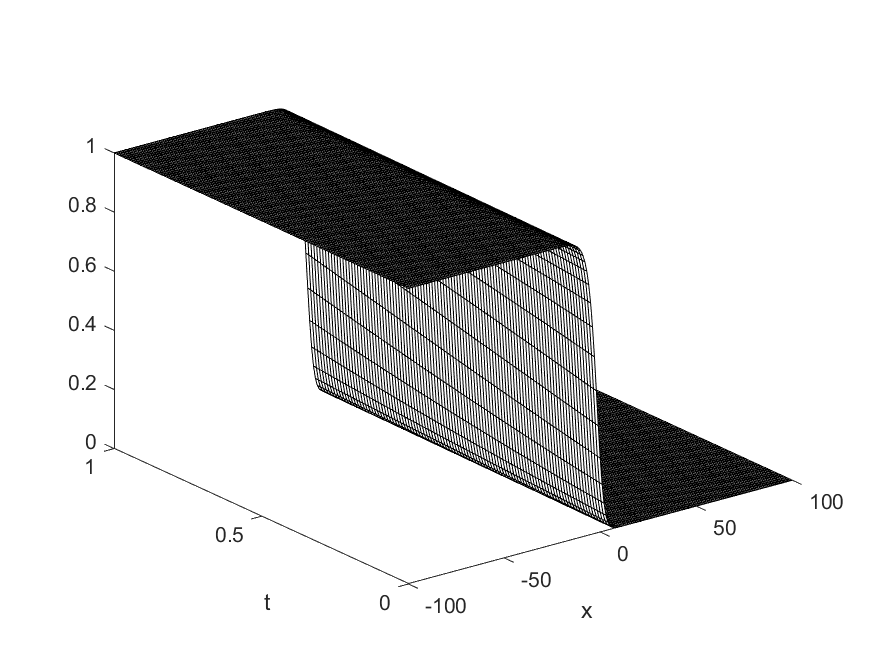
\includegraphics[scale=0.5]{problem2i1.PNG}
        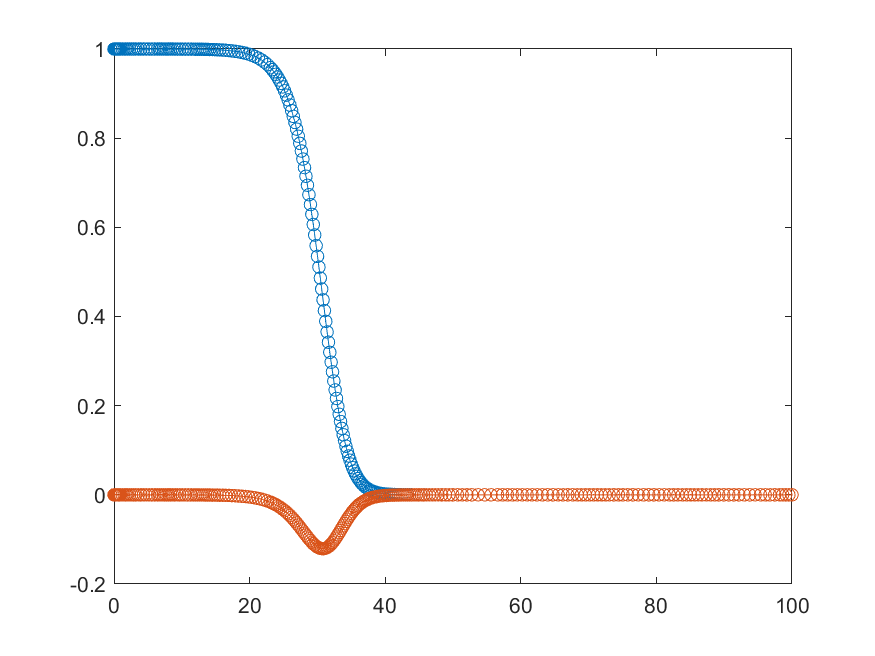
\includegraphics[scale=0.5]{problem2i2.PNG}
    \end{center}

\end{solution}

\newpage
\lstinputlisting{problem2i.m}
\newpage